\documentclass[9pt,twoside,lineno]{pnas-new}
% Use the lineno option to display guide line numbers if required.

\templatetype{pnasresearcharticle}
\usepackage{longtable}
\usepackage{array,ragged2e} % for nicer justification of table entries with "P"
\newcolumntype{P}[1]{>{\RaggedRight\arraybackslash}p{#1}}
\usepackage{caption} % for subfigures
\usepackage{subcaption}
\usepackage{lscape} % for turning one page to landscape

\let\thefigureWithoutS\thefigure %% <- store old definition
\renewcommand\thefigure{S\thefigureWithoutS}

\title{Supporting information}
\author{}
% \correspondingauthor{Corresponding Author name.\\E-mail: author.two@email.com}

\begin{document}

\maketitle 

\section{Supporting information text}

% \subsection*{Subhead}
% Type or paste text here. This should be additional explanatory text such as an extended technical description of results, full details of mathematical models, etc.   
\subsection{Sensitivity analyses for identifying introductions}
Here we describe different sensitivity analyses we performed for the definition of an introduction. 

\subsubsection{Number of focal Swiss sequences analyzed}
To assess whether the number of identified introductions saturates as we add more sequences, we did a sub-sampling analysis. We sub-sampled the Swiss genome sequences used in our main analysis from 5\% of confirmed cases down to 1\% of confirmed cases. For each new sub-sampling value, we calculated the number of introductions (singletons and transmission chains) that we would have identified given the sub-sampled sequence set. Figure \ref{fig:sensitivity_figs}a shows that as we add sequences, we do not reach saturation. Therefore, if we were to include even more sequences, we would almost certainly identify more introductions into Switzerland.

\subsubsection{Ratio of foreign context to focal Swiss sequences analyzed}
Next, we assessed how summary statistics about identified introductions and the runtime of our pipeline changed as we added more and more foreign context sequences. We kept the number of focal Swiss sequences constant at 5\% of confirmed cases each week and added foreign context sequences at a 1:1, 2:1, and 3:1 ratio to focal Swiss sequences. Figure \ref{fig:sensitivity_figs}b shows that as we add foreign context sequences, we identify more numerous, smaller introductions. However, the greatest differences come from the different assumptions about how to resolve polytomies (few vs. many introductions), not the ratio of foreign context to focal Swiss sequences. Therefore, we chose to present results using the 2:1 ratio to balance speed (smaller dataset = faster tree search convergence) and information content (larger dataset = more precise estimates of introduction dates).

\subsubsection{Criteria for identifying introductions}
After deciding on a ratio of foreign context to focal Swiss sequences, we assessed how summary statistics about identified introductions changed depending on the precise heuristic definition of an introduction. Given phylogenetic trees with polytomies, we picked transmission chains off of these trees as described in the main text methods. Here, we varied (a) the number of export events allowed in each transmission chain and (b) the maximum number of export events allowed to occur along each single internal branch. Figure \ref{fig:sensitivity_figs}c shows that increasing (a) yields fewer, larger transmission chains. Increasing (b) for each level of (a) has a much smaller effect. We note that again, the greatest differences come from the different assumptions about how to resolve polytomies. Therefore, we chose to present results using a transmission chain definition based on (a) maximum 3 exported lineages and (b) maximum one consecutive export on each internal branch. This allows for some exports from Swiss transmission chains but not arbitrarily many. 

\subsection{Sensitivity analyses for phylodynamic modelling}
Here we describe different sensitivity analyses we performed for our phylodynamic analysis.

\subsubsection{Sampling proportion prior}
First, we wanted to check that our phylodynamic estimates of a transmission damping factor are robust to our prior on the sampling proportion. Therefore, we repeated our analyses using two different priors on the sampling proportion. The first prior was a uniform distribution between 0 and 1. This broad prior allows the sampling proportion to assume any plausible value. The second prior was a uniform distribution between 0 and an upper bound equal to the number of genome sequences analyzed in a week divided by the number of confirmed cases that week. This narrower prior assumes that there are at least as many cases each week as confirmed cases. Figure \ref{fig:ReSampProbResults}a shows that in Switzerland, the estimated sampling proportion in late Fall 2020 varies greatly depending on the prior. A drop in SARS-CoV-2 diversity in Switzerland during this period might explain why the inference under the broader sampling prior estimates a proportion corresponding to fewer individuals than we know were infected during this time. Figure \ref{fig:ReSampProbResults}b shows that the effective reproductive number estimates in Fall 2020 for Switzerland more closely match estimates based on line-list data when the sampling proportion is treated as a fitting parameter, i.e. under the first, broad prior. Therefore, we report results under this prior in the main text. In Figure \ref{fig:DampingFactorResults}a, we show that the damping factor results are qualitatively similar between the two sampling proportion priors. 

\subsubsection{Population structure: a class of individuals with more contacts}
Next, we wanted to check if our transmission damping factor estimates might be due to individuals returning from travel having more dense contact networks than the general population. Therefore, we repeated our analysis for Switzerland including an additional class of infected individuals who transmit at a higher rate. Let $\pi_N$ be the fraction of normal individuals in the population and $\pi_{SS}$ be the fraction of individuals who have more contacts. Then, the $\pi_{SS}$ fraction of individuals transmit according to the background time-varying reproductive number multiplied by an additional positive factor $r_{SS}$. The parameters $\pi_N$, $\pi_{SS}$, and $r_{SS}$ were all inferred in this analysis. Figure \ref{fig:InflationFactorResults} shows that a significant fraction of the population (approximately 10-20\%) is estimated to transmit at a higher rate (over approximately 1.8 times as much). But even with the inclusion of this second deme of individuals in the model, Figure \ref{fig:DampingFactorResults}b shows that the damping factor estimates are quite stable.

\subsection{Logged trees}
Finally, we logged phylogenetic trees for a few introductions. These trees were sampled by the Markov chains in the phylodynamic analyses. Note that the damping factor results are jointly inferred from all the branching events across introductions in each time period. But since logging all introductions would yield huge log files, we logged just a few individual introductions under each set of model assumptions for visual inspection. For each set of model assumptions and each month, we logged trees for the 50th and 95th percentile largest introductions that were first sampled that month and eventually yielded > 2 samples. Figure \ref{fig:logged-chains} shows as an example summary trees for these introductions under the phylodynamic analysis for Switzerland with an un-bounded sampling proportion prior and a homogeneous population (no class of individuals with more contacts).

\section{Supporting information figures}

\begin{figure}[h!]
\centering
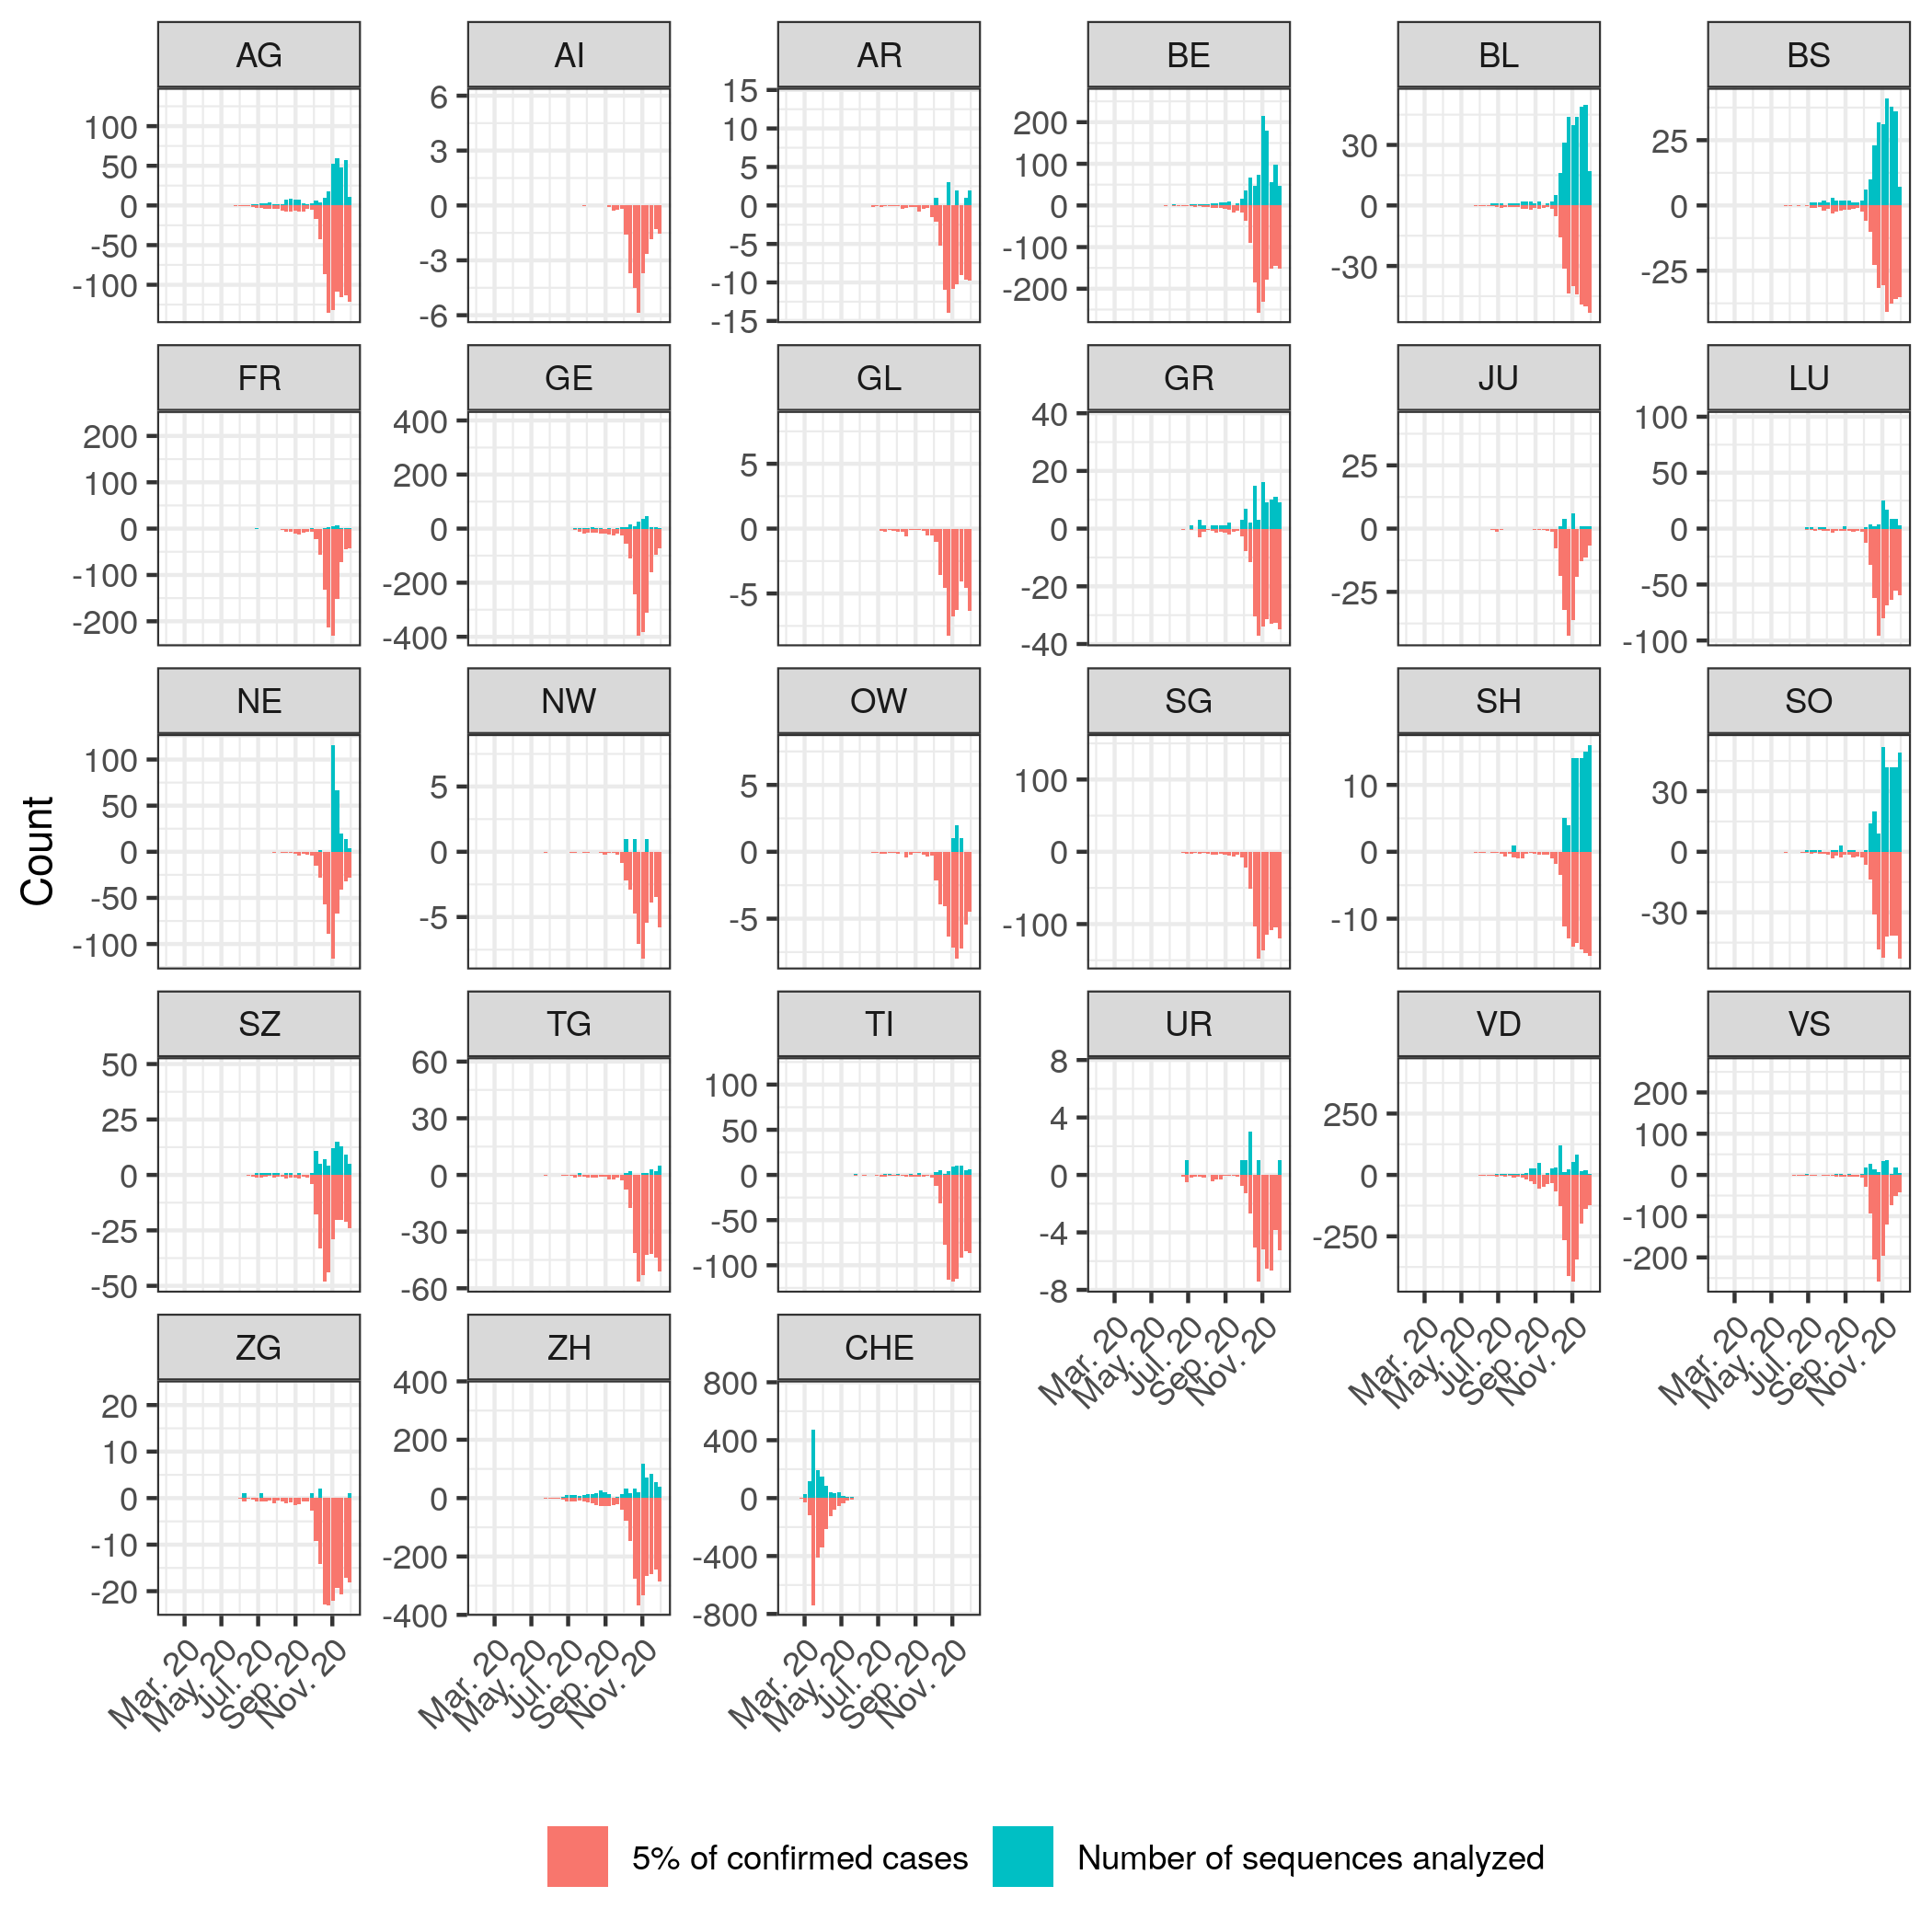
\includegraphics[width = 0.8\linewidth]{figures/CHE_downsampling.png}
\caption{Spatio-temporal representativeness of analyzed genome sequences. The mirror y-axis aims to contrast temporal trends in confirmed cases (red) versus analyzed sequences (blue); all values are positive counts. Facet titles are standard abbreviations for Swiss cantons. 'CHE' represents Swiss-wide cases and sequences, since case count reporting by canton began mid-May 2020.}  
\label{fig:downsampling_representativeness}
\end{figure}

\begin{figure}[h!]
\centering
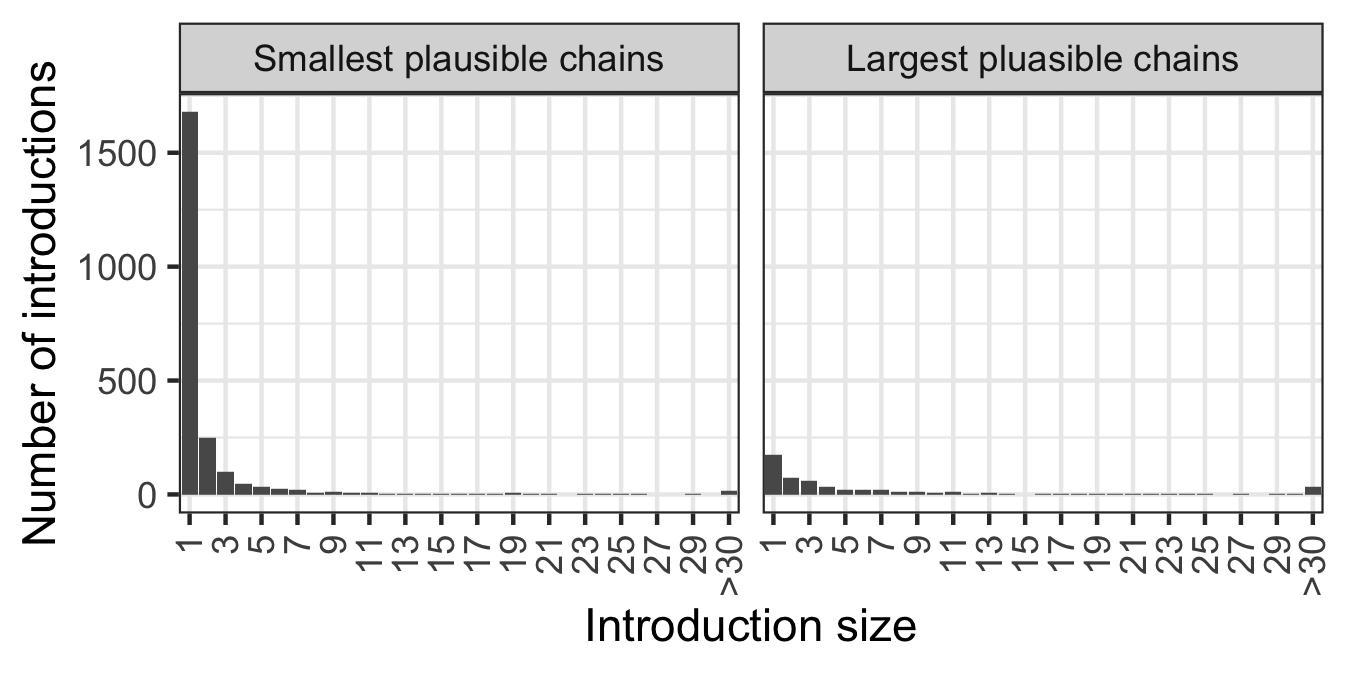
\includegraphics[width = 0.5\linewidth]{figures/chain_size_dist.png}
\caption{Size distribution of estimated introductions.}  
\label{fig:chain_size_dist}
\end{figure}

\begin{figure}[h!]
\centering
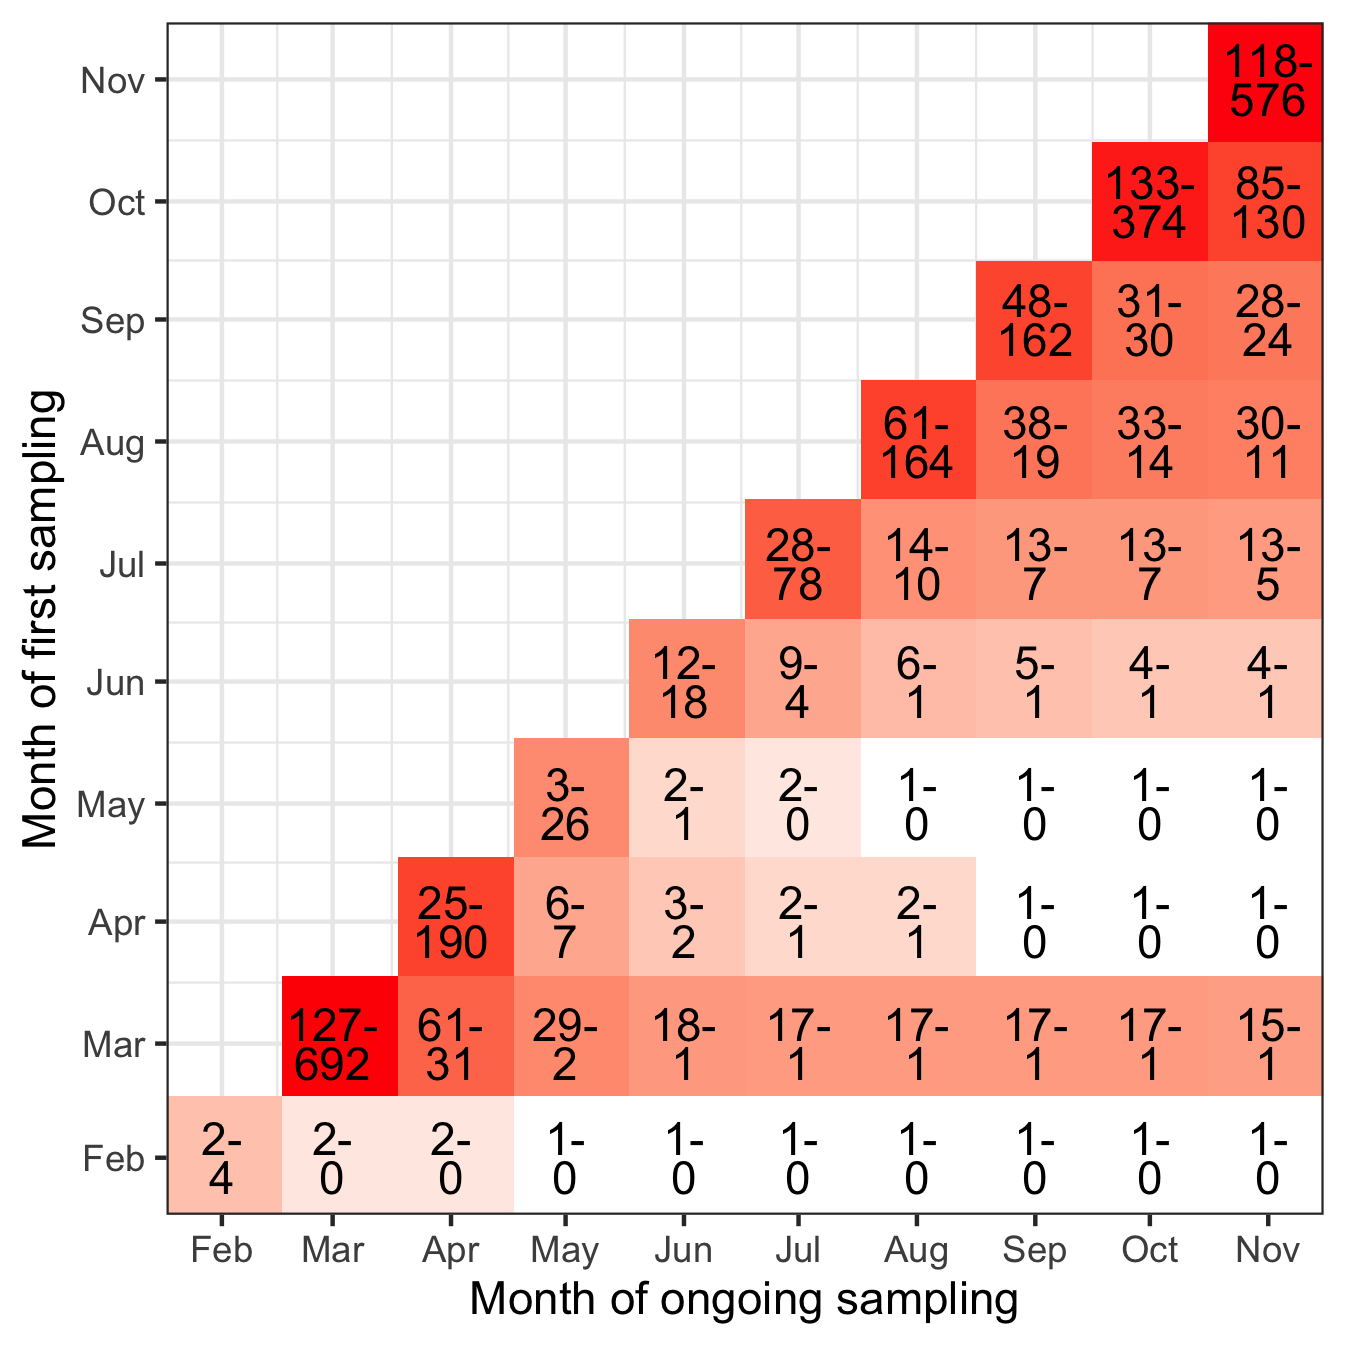
\includegraphics[width = 0.5\linewidth]{figures/chain_longevity_matrix.png}
\caption{Heatmap of the number of newly sampled introductions in Switzerland each month (diagonal entries) and the number continuing to persisting into each following month (off-diagonal entries). Introduction are counted once in the month they are first sampled (``Month of first sampling'') and one every following month (``Month of ongoing sampling'') until the date of the latest sample. The ranges are between two point estimates generated assuming either few or many introductions.}  
\label{fig:chain-longevity-matrix}
\end{figure}

\begin{figure}[h!]
\centering
\begin{subfigure}[b]{\textwidth}
\centering
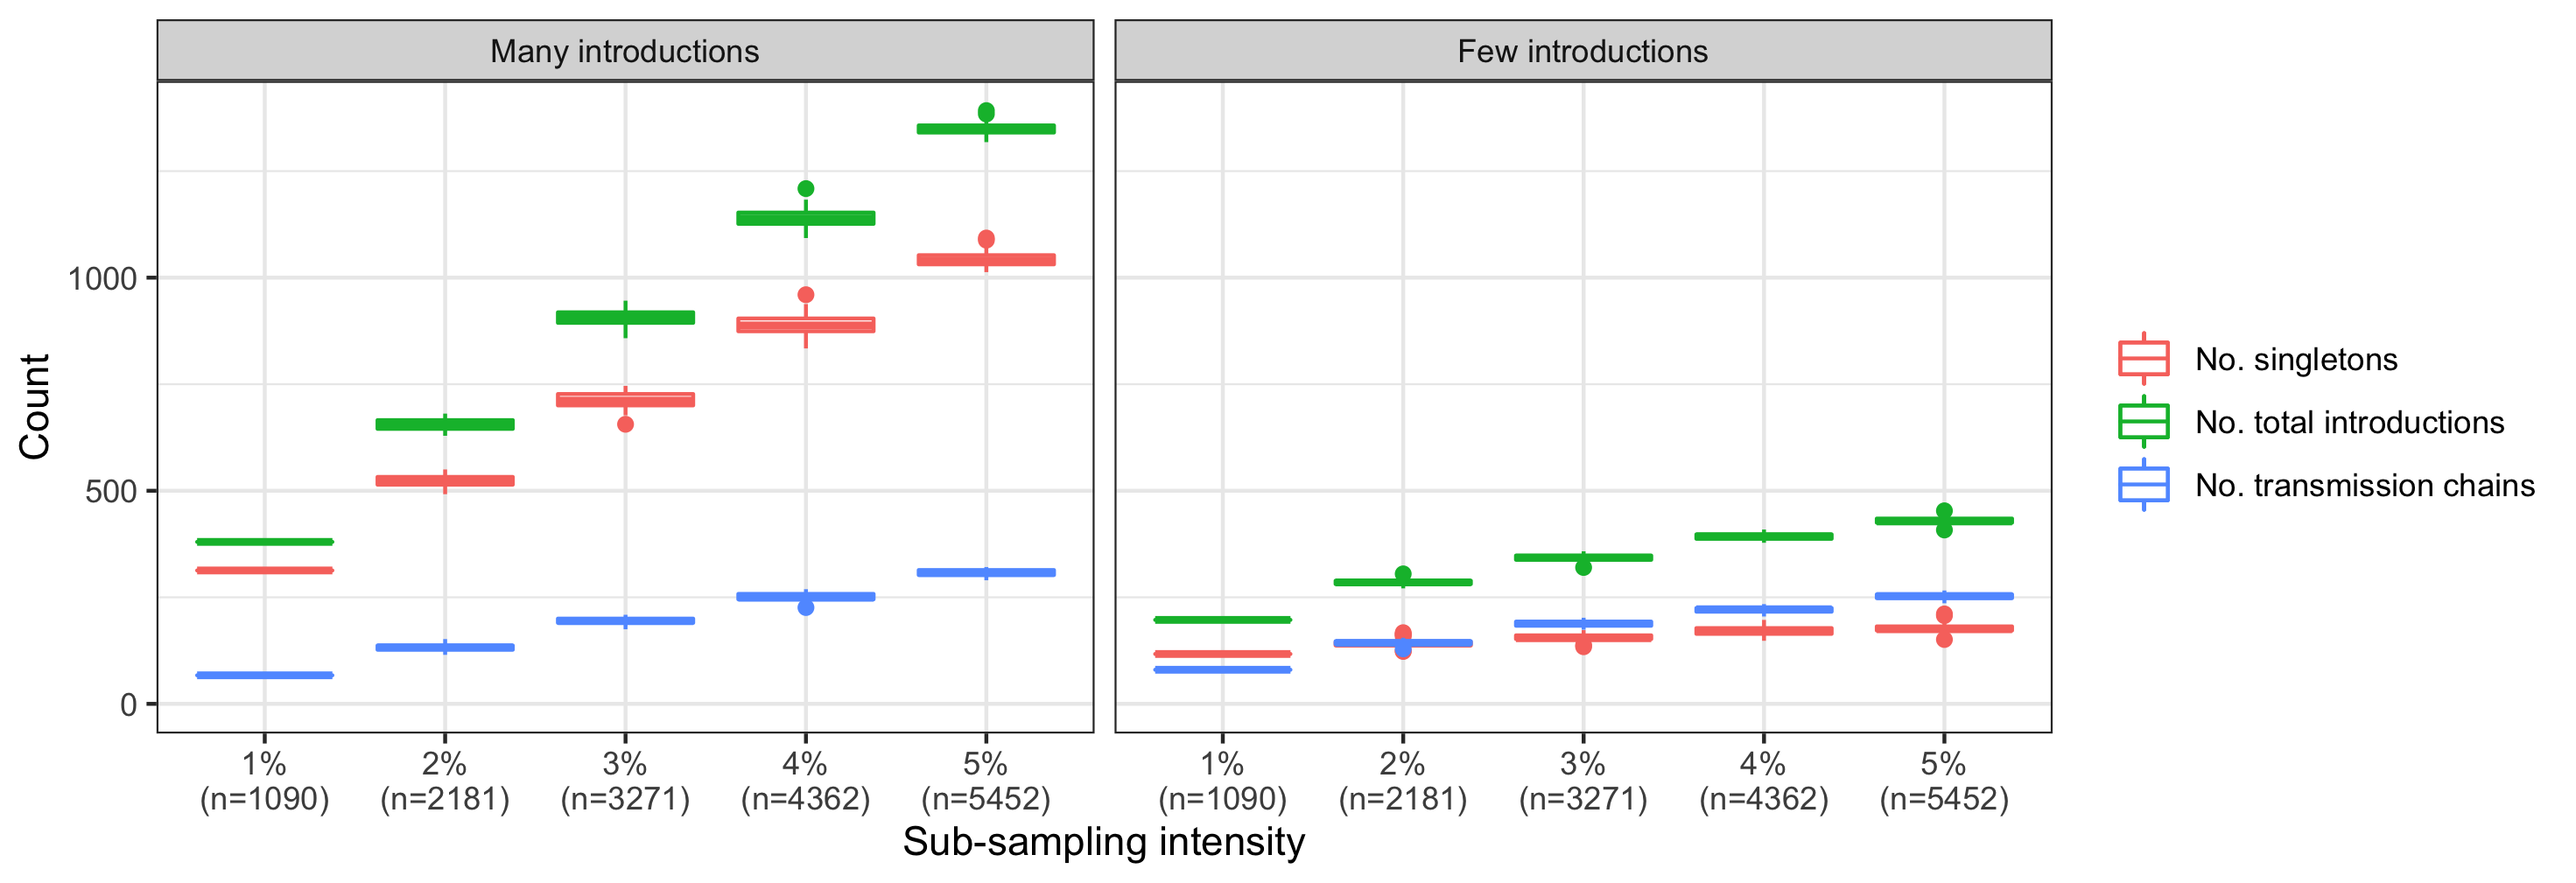
\includegraphics[width = 11.4cm]{figures/fig_SX_sensitivity_subsampling.png}
\caption{Estimated introductions by percent (or, n=number) of Swiss confirmed cases analyzed. No. = number. Each box plot is a summary over 50 random sub-samples.}  
\end{subfigure}

\begin{subfigure}[b]{0.9\textwidth}
\centering
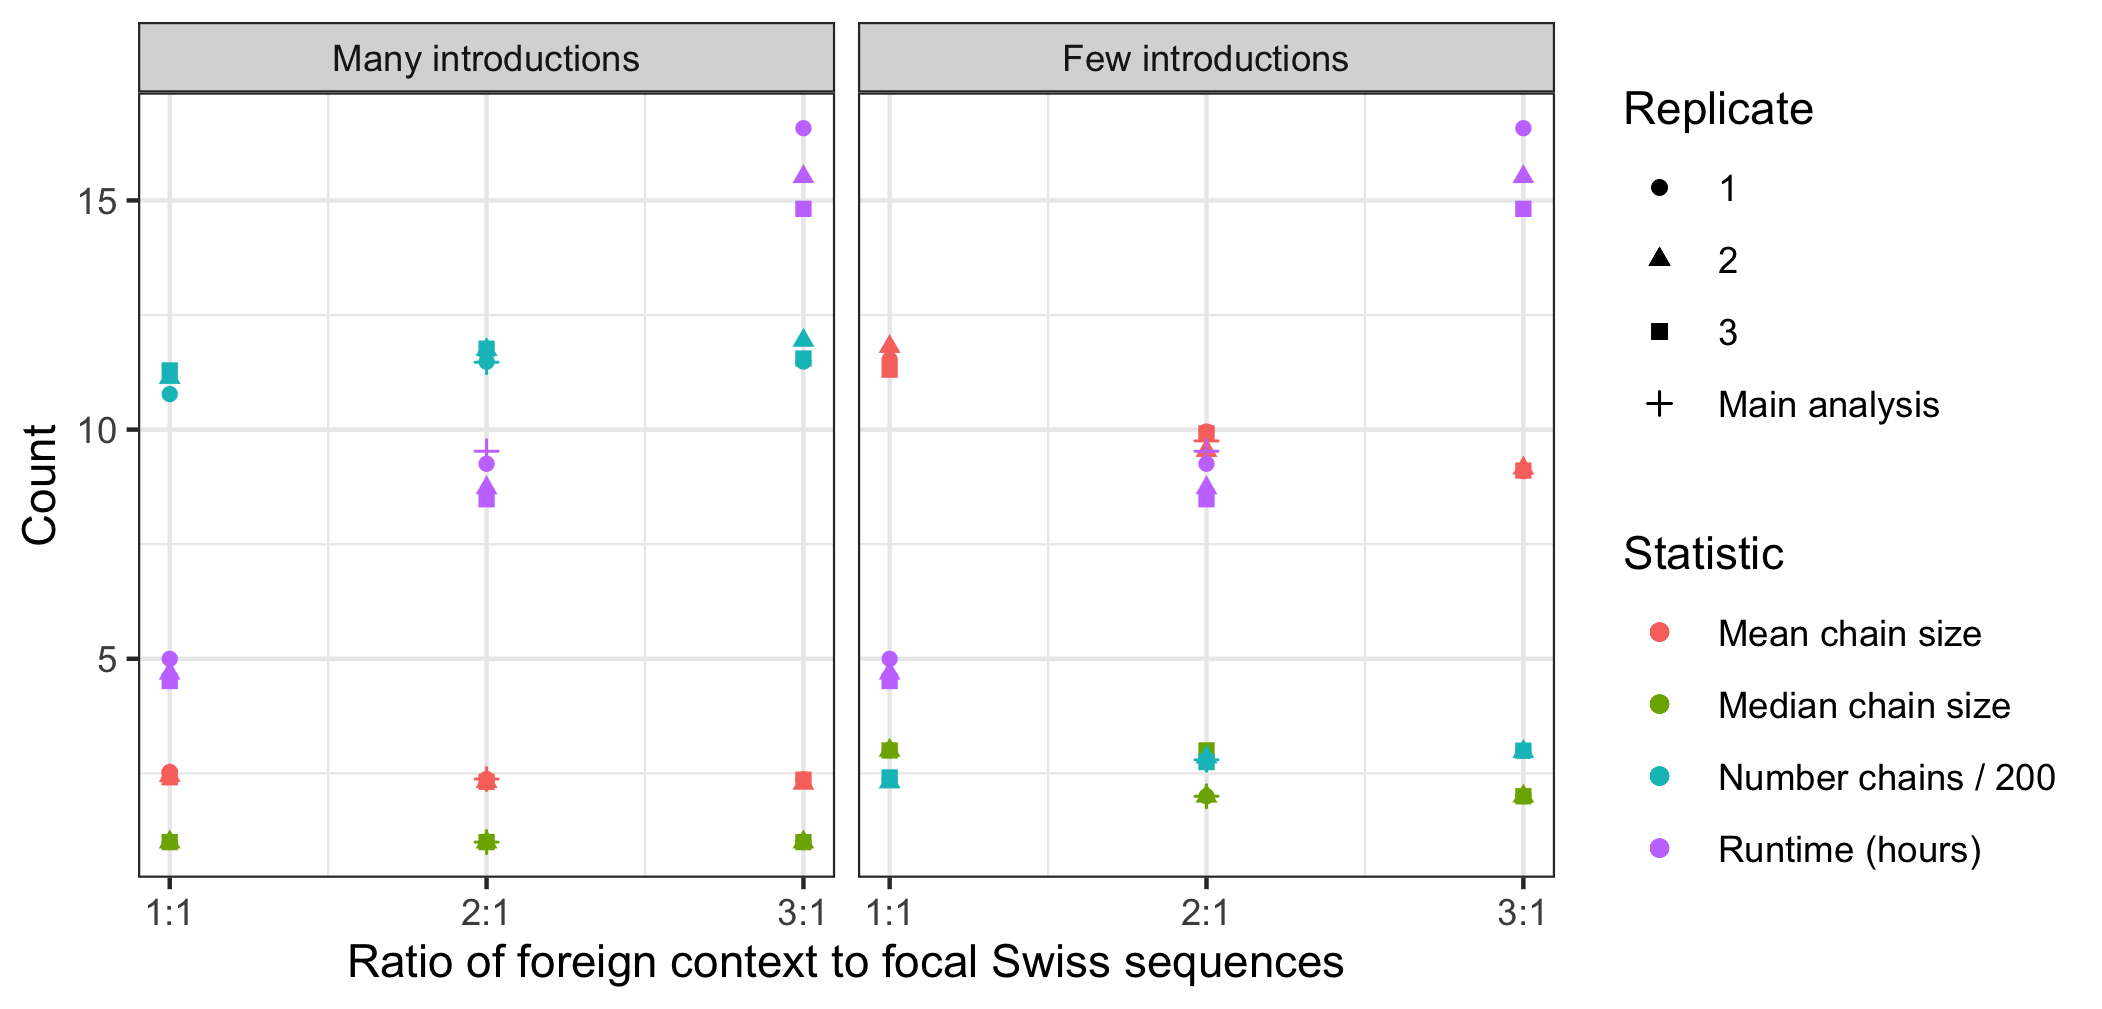
\includegraphics[width = 11.4cm]{figures/fig_SX_sensitivity_context_set_size.png}
\caption{Summary statistics about introductions by ratio of foreign context to focal Swiss sequences.}  
\end{subfigure}

\begin{subfigure}[b]{0.9\textwidth}
\centering
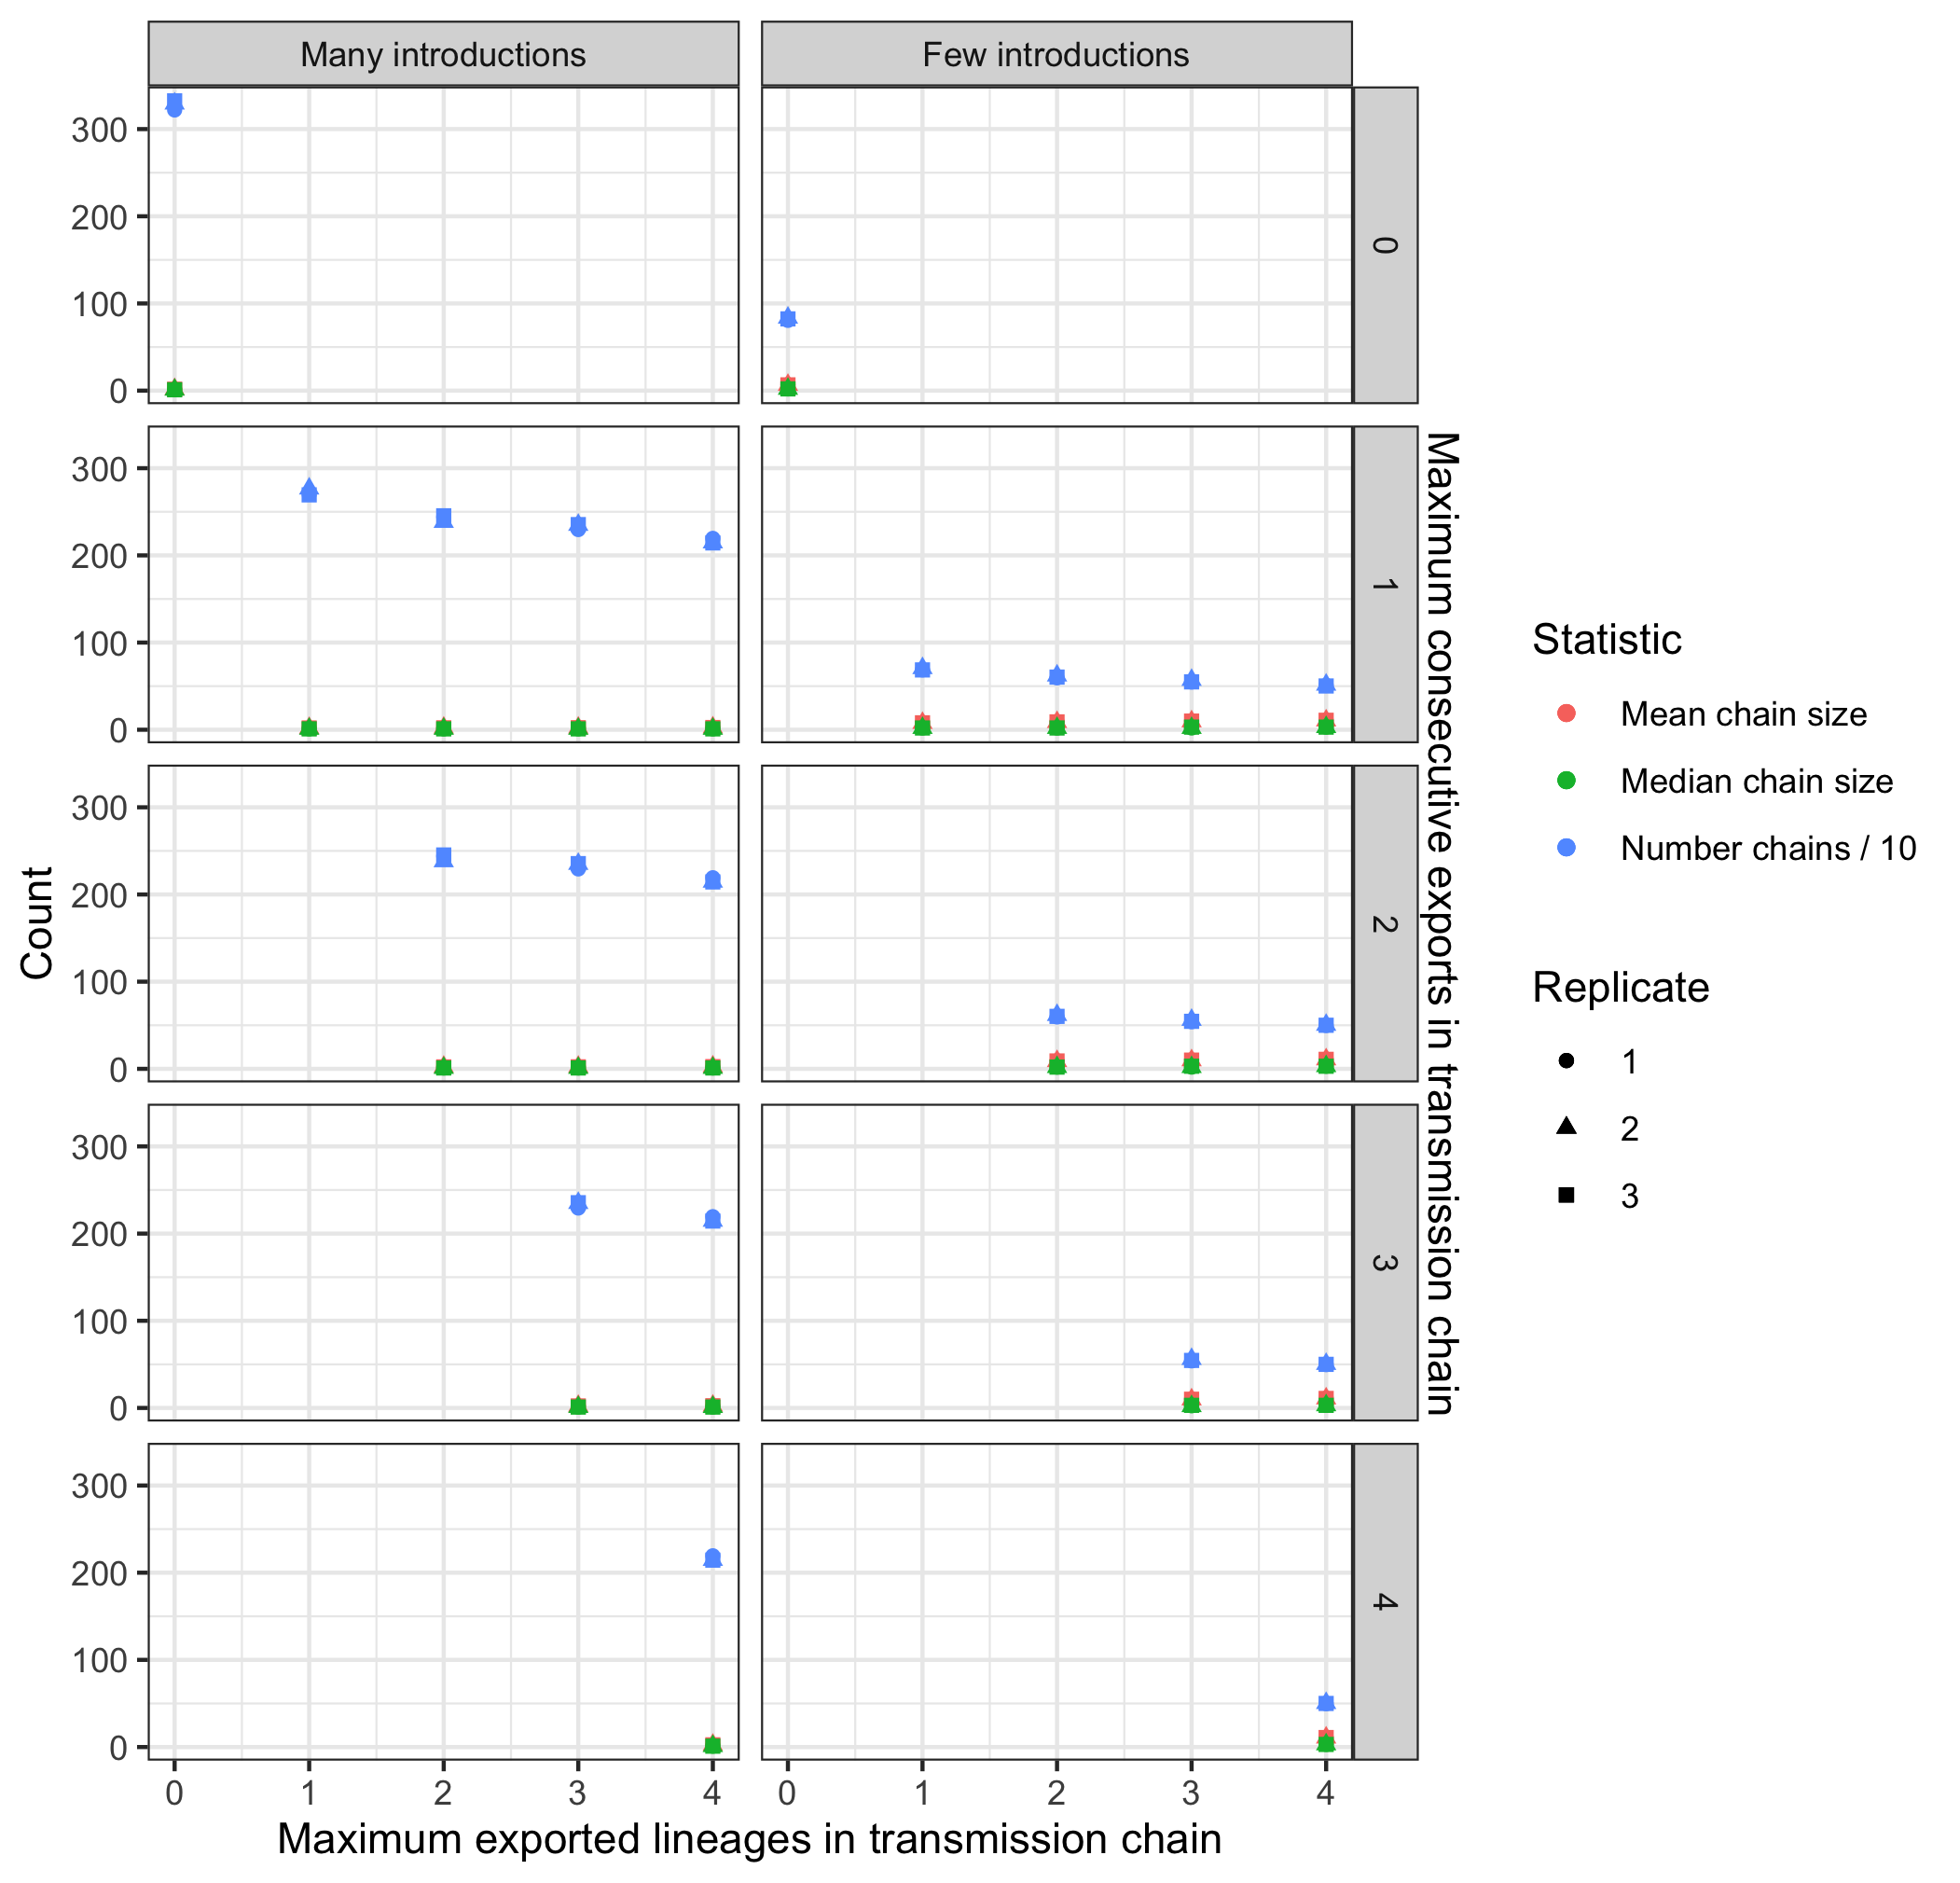
\includegraphics[width = 11.4cm]{figures/fig_SX_sensitivity_chain_defn.png}
\caption{Summary statistics about introductions and pipeline runtime by different heuristic definitions of an introduction.}  
\end{subfigure}
\caption{Sensitivity analyses for the definition of an introduction. (a) shows sensitivity to number of focal sequences analyzed, (b) shows sensitivity to the ratio of foreign context to focal sequences analyzed, and (c) shows sensitivity to the heuristic thresholds used to define an introduction given a tree. All statistics were generated under two different polytomy assumptions giving rise to either many or few introductions.}
\label{fig:sensitivity_figs}
\end{figure}

% \begin{landscape}
\begin{figure}[h!]
\centering
\begin{subfigure}[b]{\textwidth}
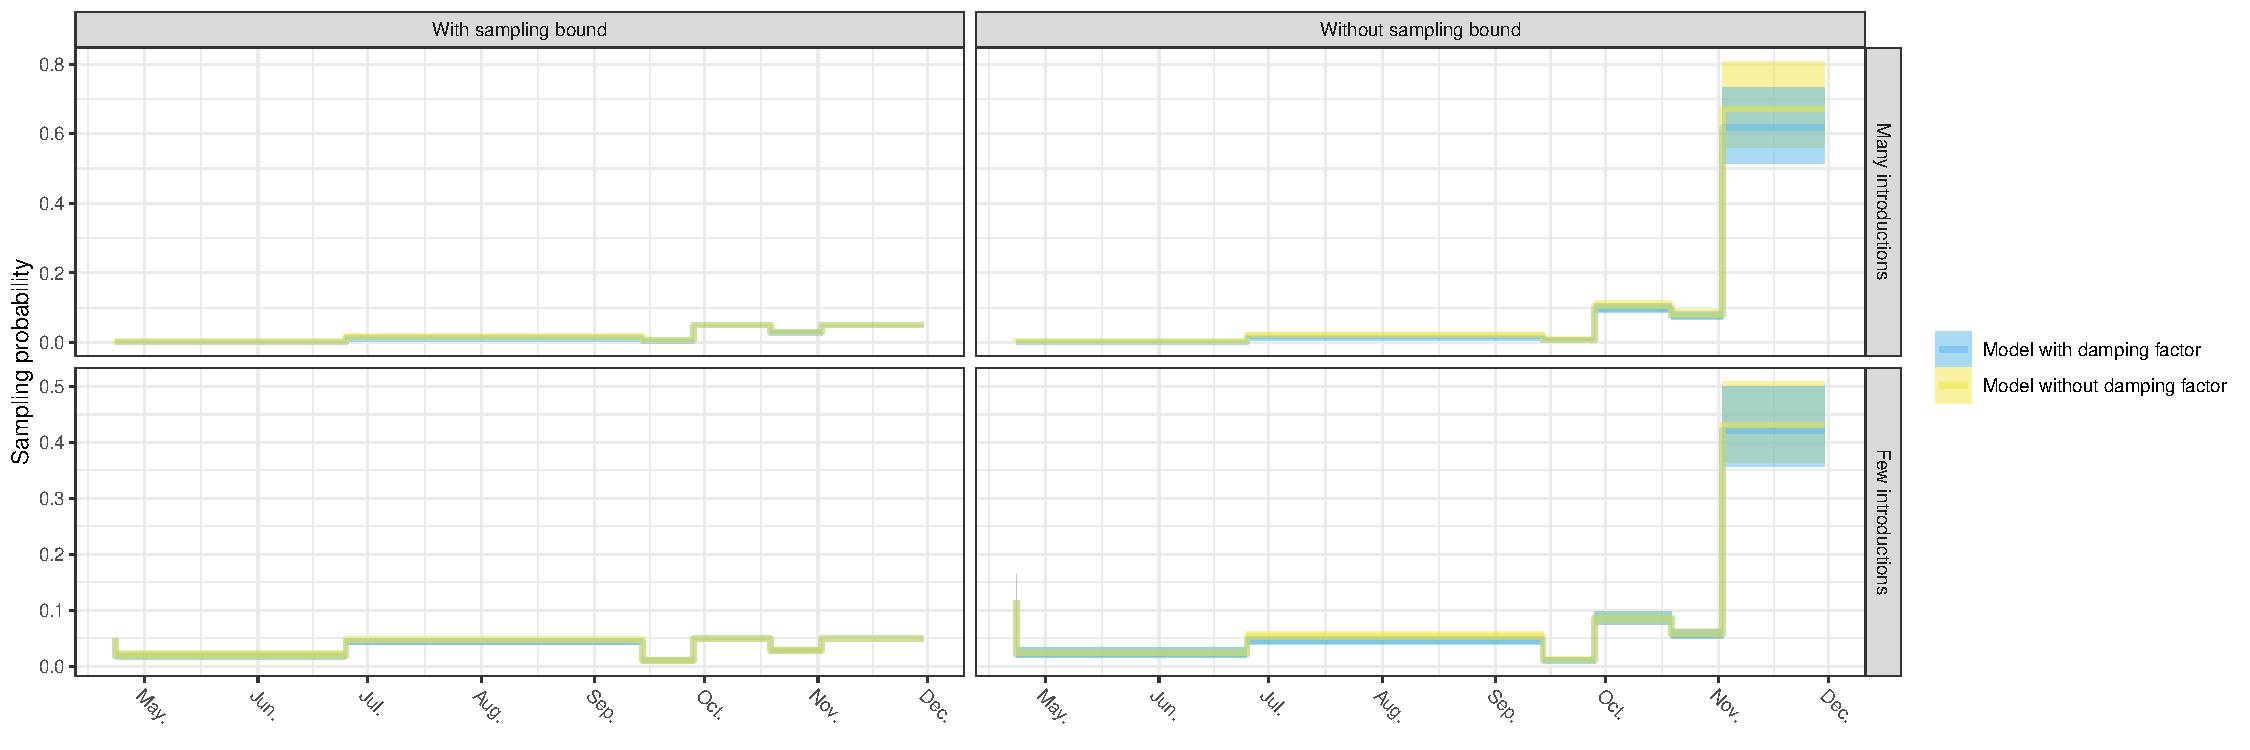
\includegraphics[width=\linewidth]{figures/CHE_sampProp.pdf}
\caption{Sampling probability in Switzerland.}
\end{subfigure}
\begin{subfigure}[b]{\textwidth}
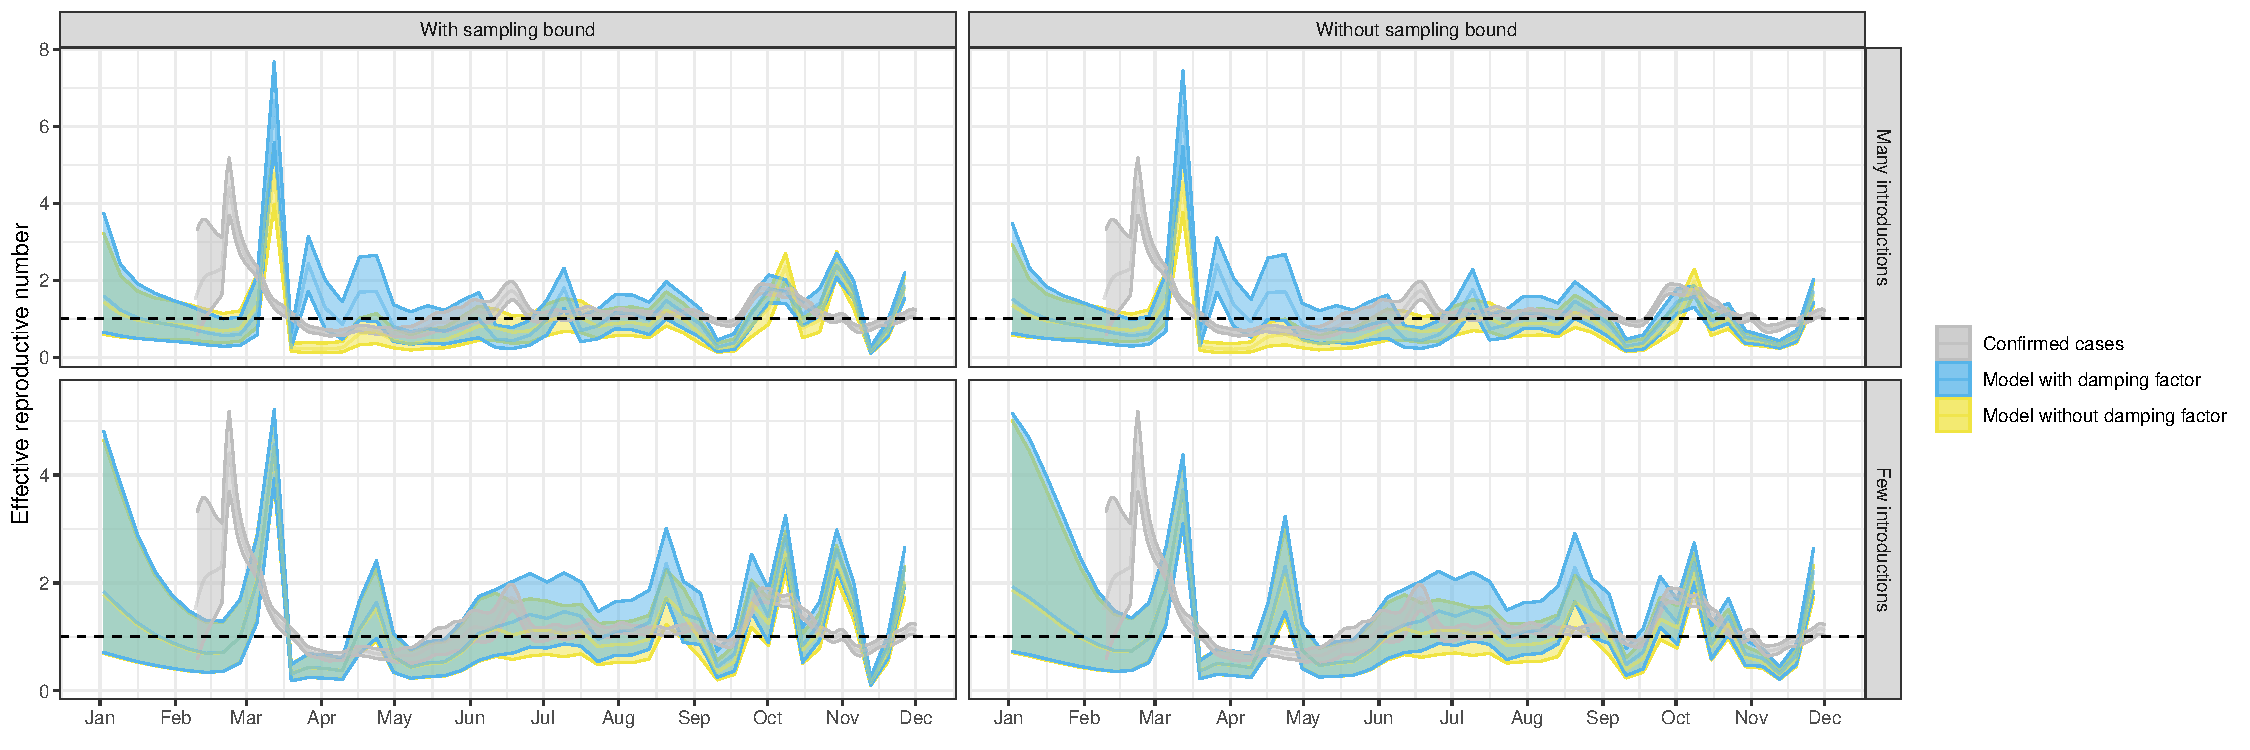
\includegraphics[width=\linewidth]{figures/CHE_Re.pdf}
\caption{Effective reproductive number in Switzerland.}
\end{subfigure}
\begin{subfigure}[b]{\textwidth}
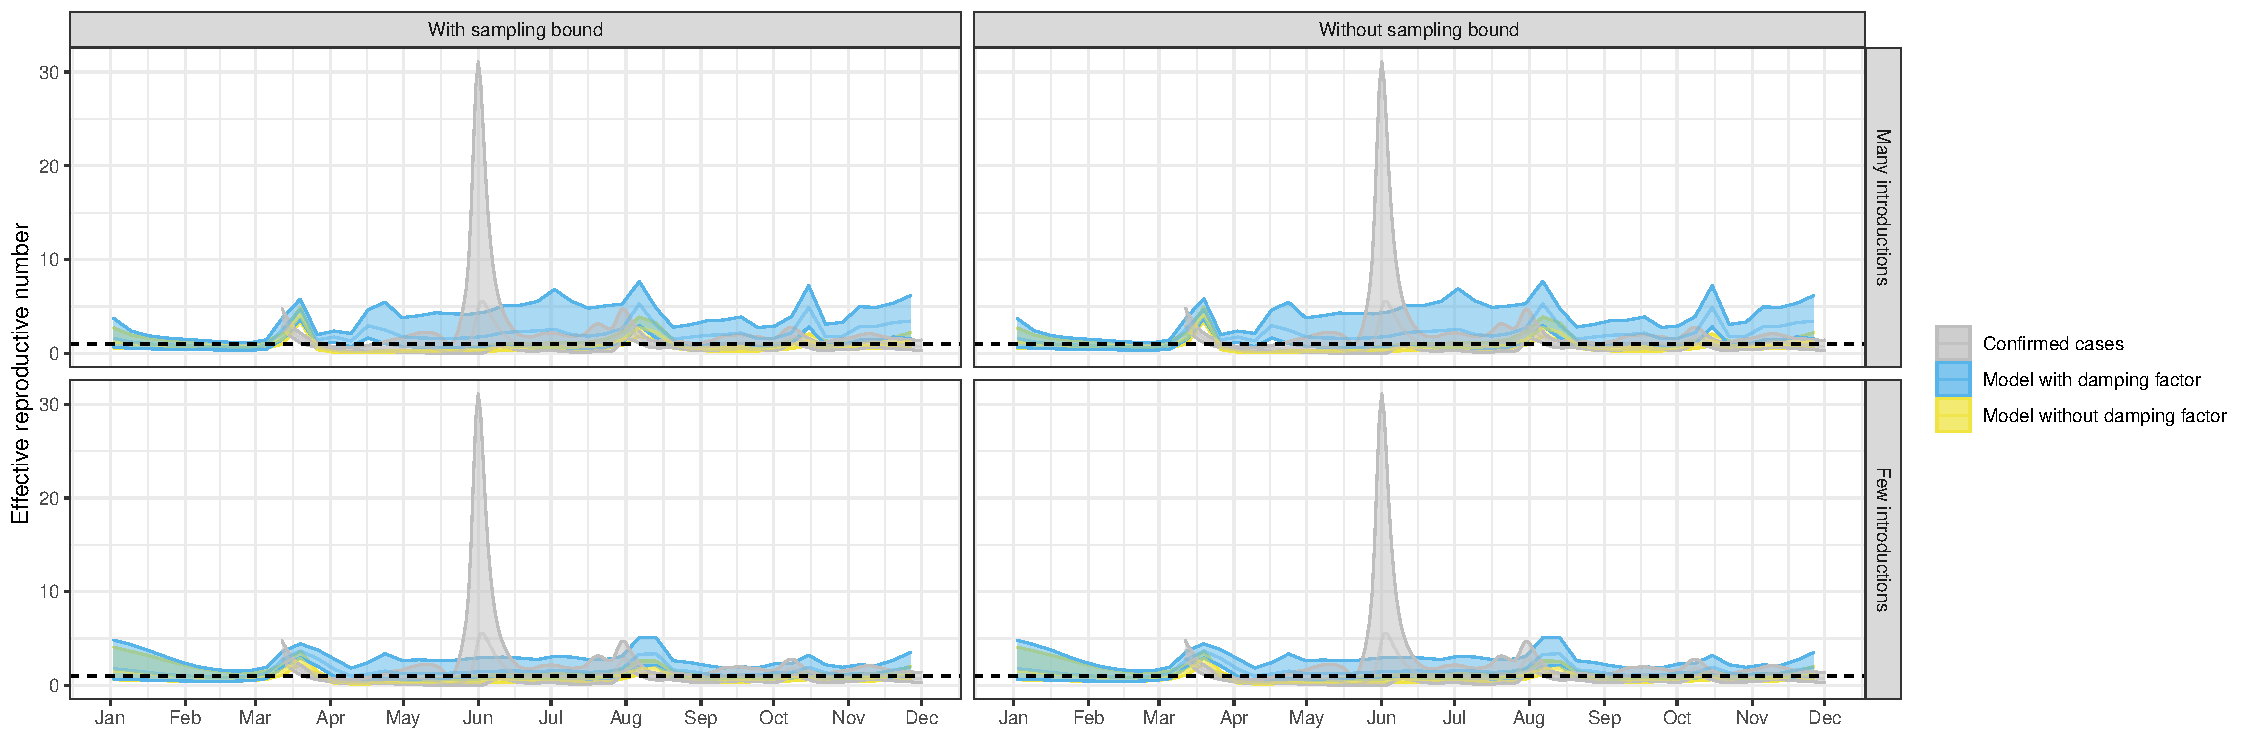
\includegraphics[width=\linewidth]{figures/NZL_Re.pdf}
\caption{Effective reproductive number in New Zealand.}
\end{subfigure}
\caption{Phylodynamic estimates for  (a) the sampling probability in Switzerland and the time-varying effective reproductive number $R_e$ in Switzerland (b) and New Zealand (c). $R_e$ estimates are overlaid on estimates generated from case count data \cite{huisman_re_preprint} in grey. Additionally, $R_e$ estimates from the models with a damping factor (pink) are the ``baseline'' $R_e$ before introduction-specific damping (i.e. before application of a damping factor once introductions are older than 2-days post sampling).}  
\label{fig:ReSampProbResults}
\end{figure}
% \end{landscape}
% Remember Re plot is now background Re (without contact tracing) and no longer the actual average Re

\begin{figure}[h!]
\centering
\begin{subfigure}[b]{0.7\textwidth}
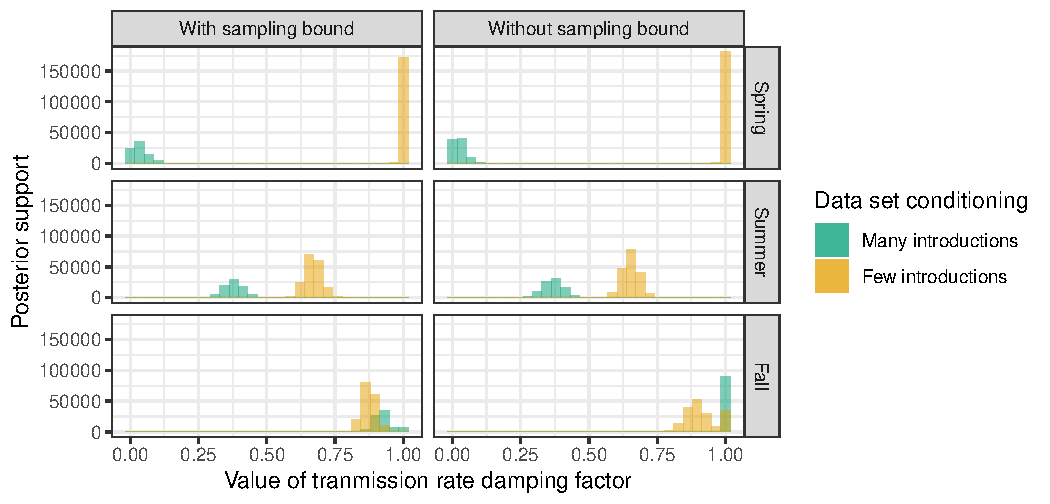
\includegraphics[width=\linewidth]{figures/CHE_contact_tracing_factor.pdf}
\caption{Damping factor in Switzerland.}
\end{subfigure}
\begin{subfigure}[b]{0.7\textwidth}
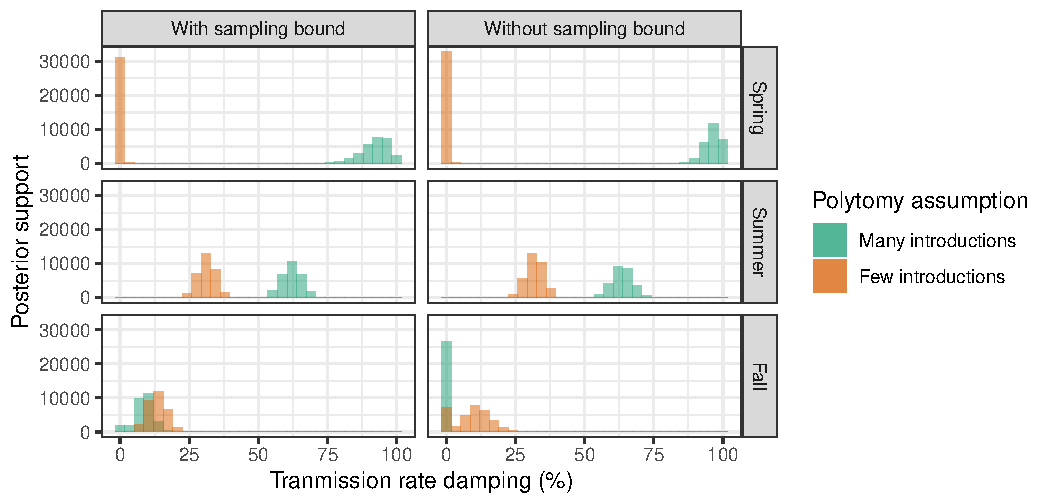
\includegraphics[width=\linewidth]{figures/CHE_2Deme_contact_tracing_factor.pdf}
\caption{Damping factor in Switzerland under 2-deme model.}
\end{subfigure}
\begin{subfigure}[b]{0.7\textwidth}
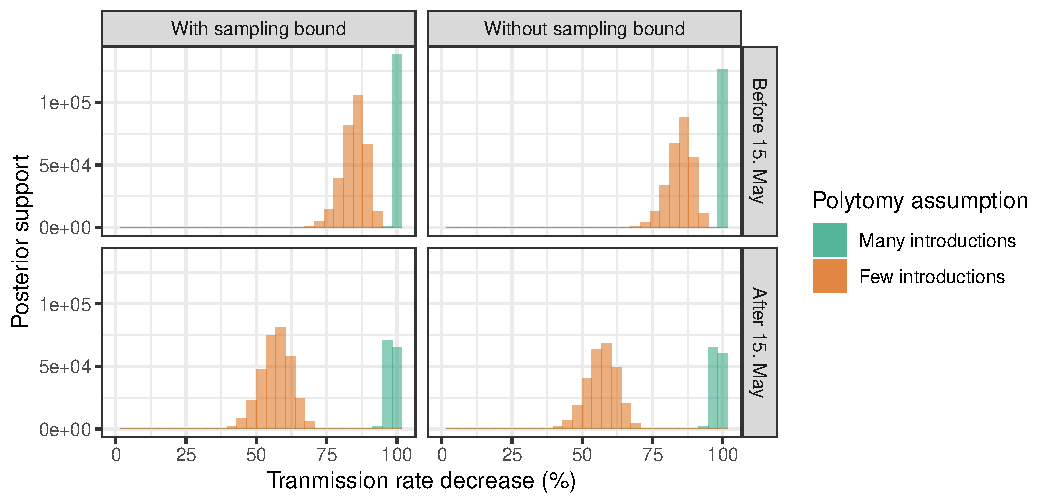
\includegraphics[width=\linewidth]{figures/NZL_contact_tracing_factor.pdf}
\caption{Damping factor in New Zealand.}
\end{subfigure}
\caption{Phylodynamic estimates for the damping factor in Switzerland and New Zealand in different time periods, conditioned on introductions defined using different polytomy assumptions and using different priors on the sampling probability.}  
\label{fig:DampingFactorResults}
\end{figure}
\newpage

\begin{figure}[h!]
    \centering
    \begin{subfigure}[b]{0.7\textwidth}
    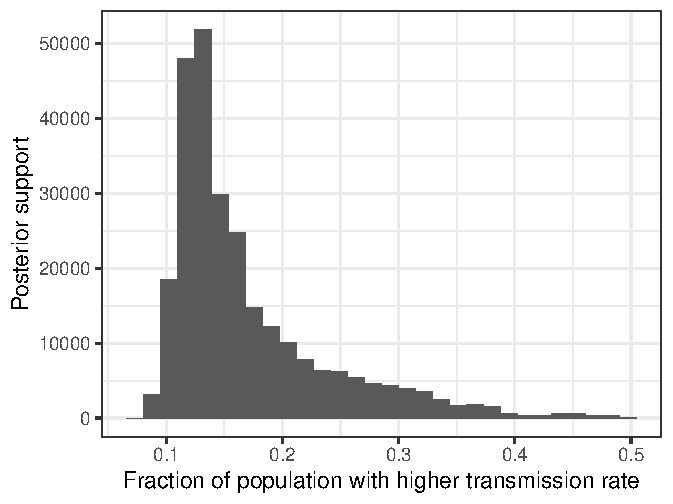
\includegraphics[width=\linewidth]{figures/CHE_2Deme_super_spreading_type_frequency.pdf}
    \caption{}
    \end{subfigure}
    \begin{subfigure}[b]{0.7\textwidth}
    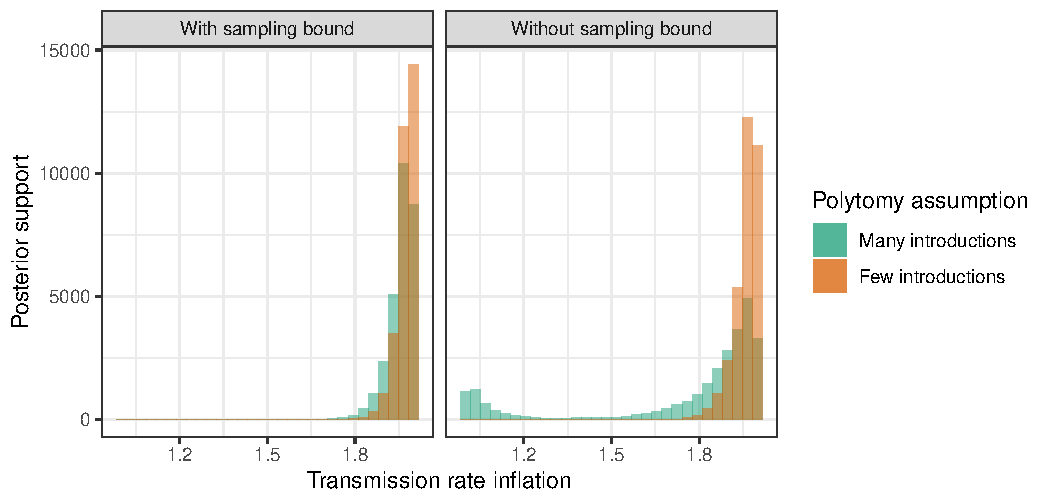
\includegraphics[width=\linewidth]{figures/CHE_2Deme_super_spreading_factor.pdf}
    \caption{}
    \end{subfigure}
    \caption{Phylodynamic estimates for (a) the fraction of the population in the deme with a higher transmission rate in Switzerland and (b) the inflation factor for the transmission rate in this deme. Estimates are shown based on conditioning on introductions defined using different polytomy assumptions and using different priors on the sampling probability.}
    \label{fig:InflationFactorResults}
\end{figure}

\begin{landscape}
\begin{figure}[h!]
\centering
\begin{subfigure}[b]{0.65\textwidth}
\centering
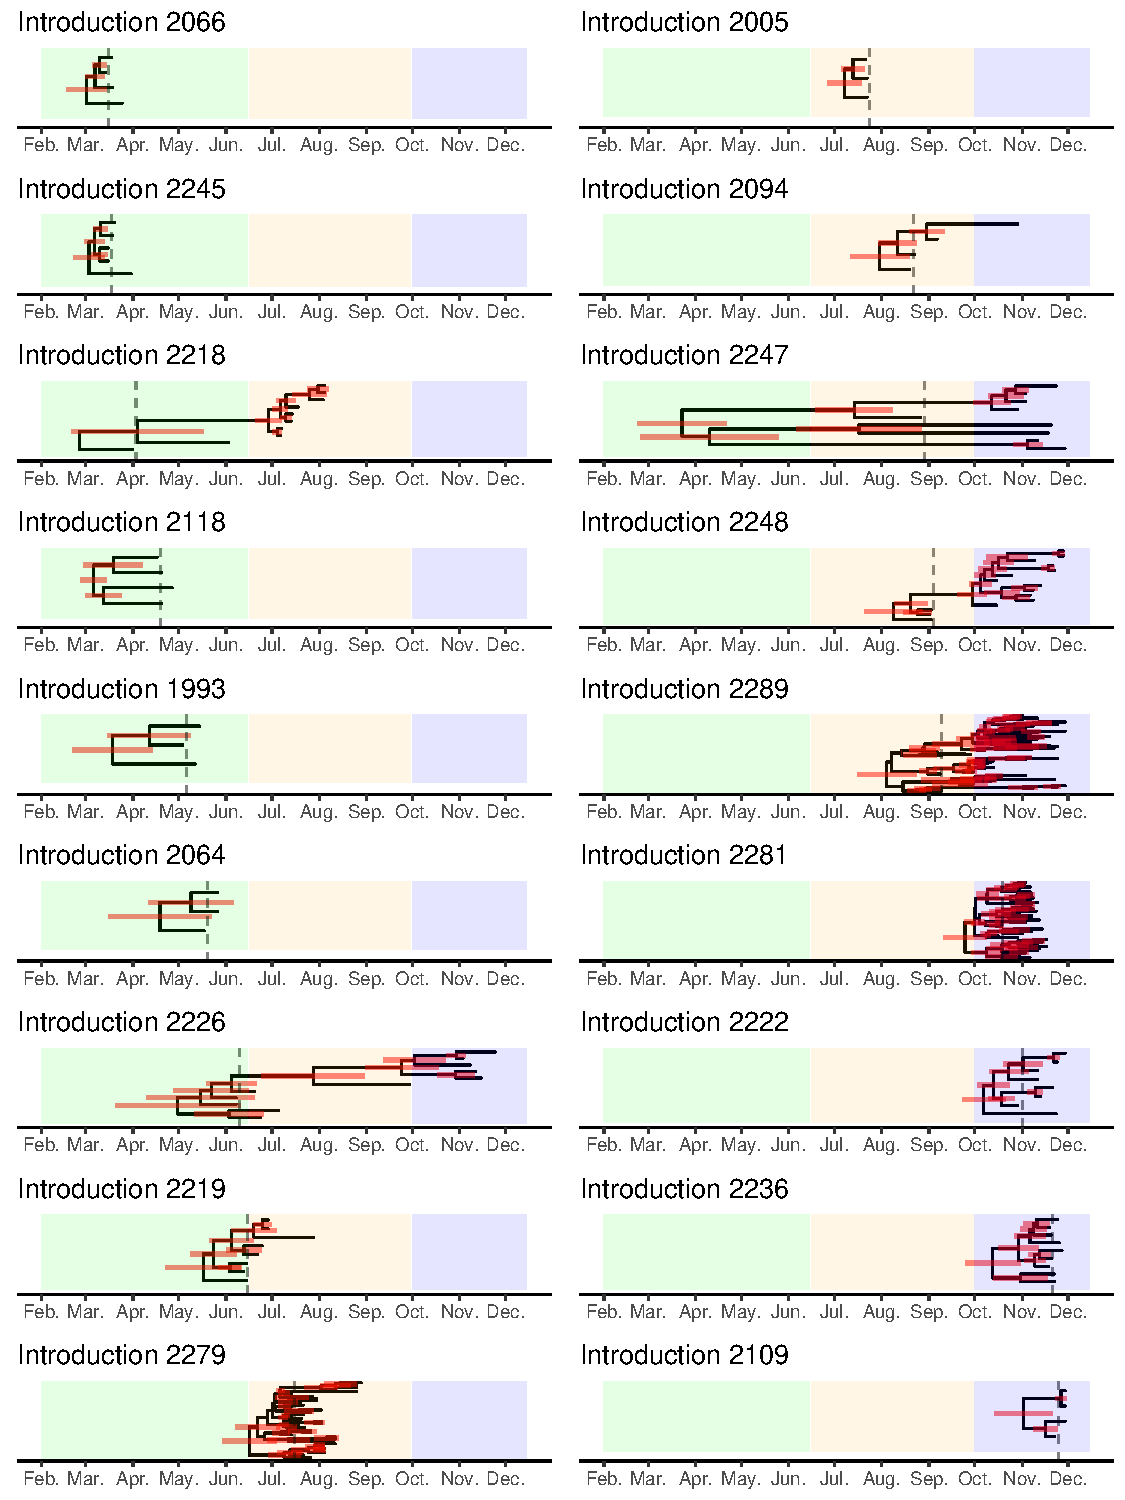
\includegraphics[width=0.75\linewidth]{figures/Re_skyline.max_chains.sampUB1.0.ctEst1.summary_trees.pdf}
\caption{Summary trees for introductions defined assuming many introductions.}
\end{subfigure}
\begin{subfigure}[b]{0.65\textwidth}
\centering
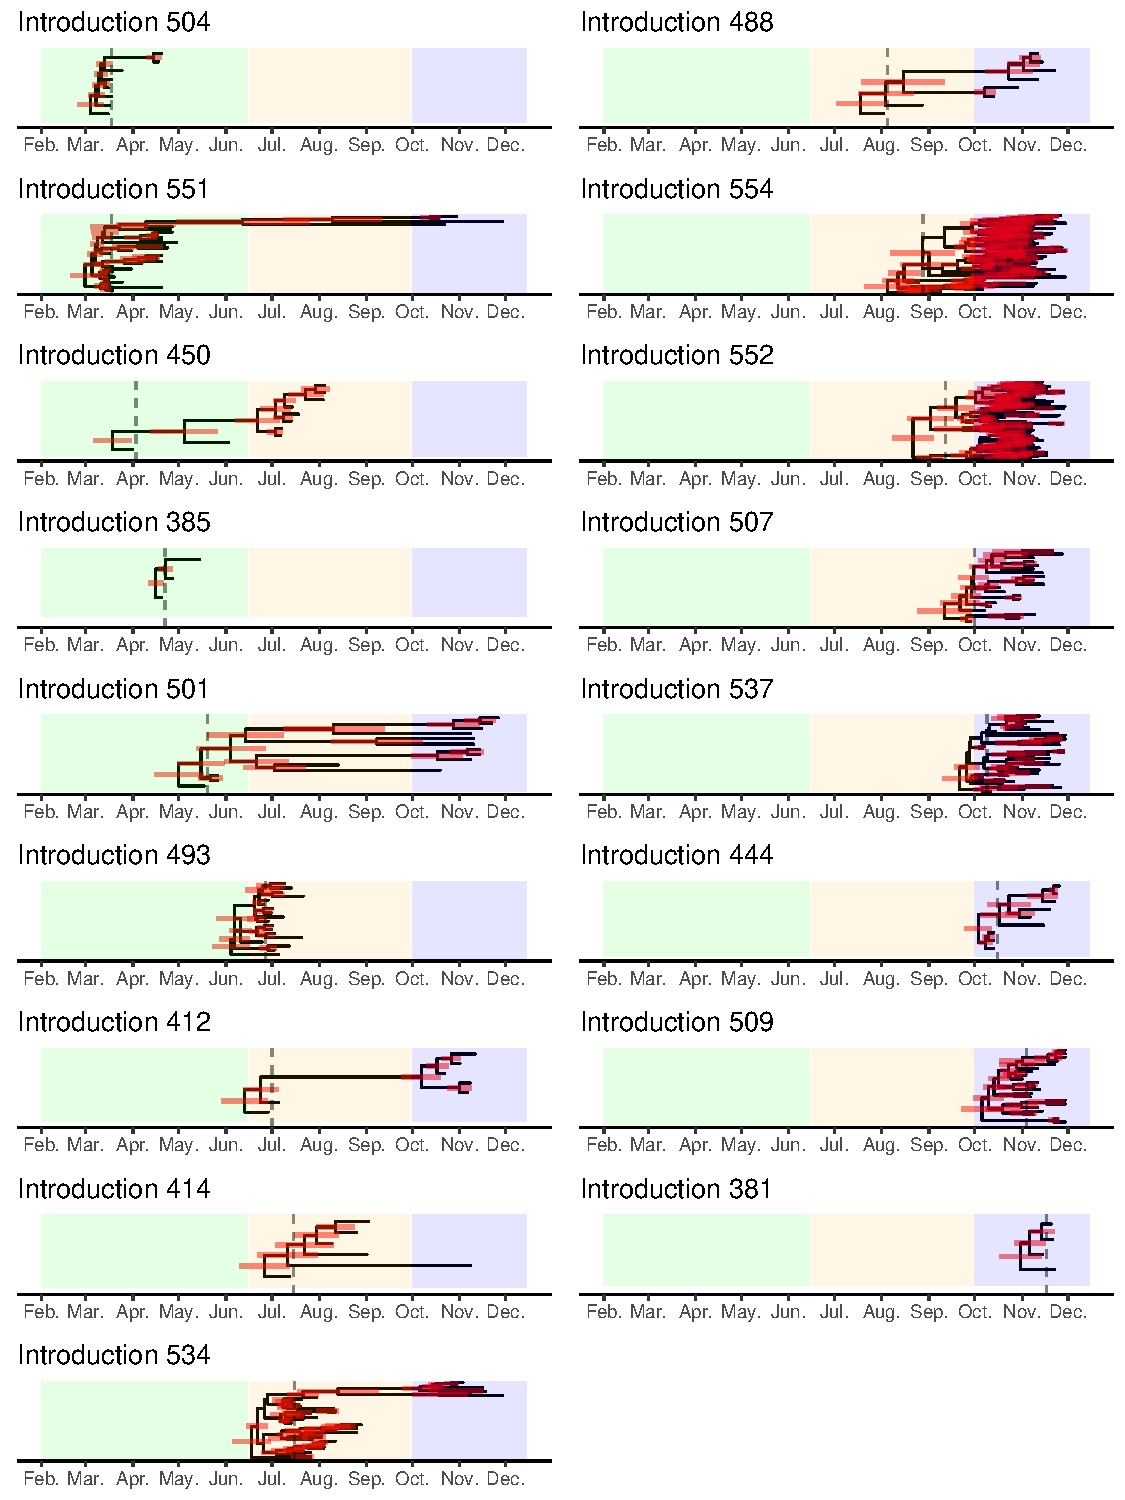
\includegraphics[width=0.75\linewidth]{figures/Re_skyline.min_chains.sampUB1.0.ctEst1.summary_trees.pdf}
\caption{Summary trees for introductions defined assuming few introductions.}
\end{subfigure}
\caption{Summary trees from the phylodynamic analysis for Switzerland. (a) and (b) show trees for introductions defined using different polytomy assumptions. The 50th and 95th percentile largest introductions among those first sampled each month are shown. The three color regions represent the Spring (green), Summer (orange) and Fall (blue) periods. The vertical dashed line shows the date at which the transmission rate can slow for each introduction - two days after the first sample date. The red bars show the 95\% highest posterior density uncertainty in node dates.}  
\label{fig:logged-chains}
\end{figure}
\end{landscape}
\newpage

\section{Supporting information tables}

\begin{table}[h!]
% \centering
\caption{Sampling proportion change-points for the phylodynamic analysis on Swiss data. The sampling proportion was modelled as a piece-wise-constant function in time, with the following change-points motivated by major shifts in the testing regime or genome sequencing intensity in Switzerland.}
\label{tab:CHE_samp_prob_change_dates}
\begin{tabular}{ll}
\hline
Start date & Description \\
\hline
23. Apr 2020 & All symptomatic individuals can get tested \\
25. Jun 2020 & Government pays for tests for symptomatic individuals \\
14. Sept 2020 & Genome sampling $<<$ 5\% of confirmed cases \\
28. Sept 2020 & Number of tests conducted and \% positivity dramatically increase, genome sampling also increases \\
19. Oct 2020 & Genome sampling $<<$ 5\% of confirmed cases again \\
11. Nov 2020 & Genome sampling improves again \\
\hline
\end{tabular}
\end{table}

\begin{table}[h!]
\caption{Contingency table for singleton introductions and transmission chains by time period assuming many (right) and few (left)  introductions.}
\label{tab:lockdown-contingency}
% latex table generated in R 4.0.5 by xtable 1.8-4 package
% Fri Sep  3 16:31:51 2021
\begin{tabular}{lcccc}
\hline
& Singleton & Transmission chain & Total \\ 
\hline
MRCA during lockdown & 533 &  91 & 624 \\ 
MRCA not during lockdown & 1209 & 461 & 1670 \\ 
Total & 1742 & 552 & 2294 \\ 
\hline
\end{tabular}

% latex table generated in R 4.0.5 by xtable 1.8-4 package
% Fri Sep  3 16:31:51 2021
\begin{tabular}{lcccc}
  \hline
 &  & Singleton & Transmission chain & Total \\ 
  \hline
1 & MRCA during lockdown &  47 &  28 &  75 \\ 
  2 & MRCA not during lockdown & 152 & 332 & 484 \\ 
  3 & Total & 199 & 360 & 559 \\ 
   \hline
\end{tabular}

\end{table}

% latex table generated in R 4.0.5 by xtable 1.8-4 package & modified manually
% Thu Aug 12 18:13:52 2021
\begin{longtable}[l]{cccP{4cm}c}
\caption{Summary of Pango lineages analyzed. If more than 50\% of the samples from a lineage in the full, quality-filtered dataset were Swiss, we aggregated them into the parent lineage. The percentage of Swiss samples in the final, aggregated lineage sets are given in column ``\% lineage Swiss''. Lineage aliases were also aggregated with their extended-form names. A separate phylogeny was constructed for each lineage analyzed.}
\label{tab:lineage-data-summary}
\hline
 & Lineage analyzed & No. Swiss samples analyzed & Lineages aggregated & \% lineage Swiss \\ 
\hline
1 & B.1.160 & 1347 & B.1.160, B.1.160.10, B.1.160.11, B.1.160.12, B.1.160.14, B.1.160.15, B.1.160.16, AB, B.1.160.19, B.1.160.20, B.1.160.22, B.1.160.26, B.1.160.29, B.1.160.30, B.1.160.31, B.1.160.32, B.1.160.9, B.1.160.16.1, AB.1 & 19.00 \\ 
  2 & B.1.177 & 1260 & B.1.177, B.1.177.23, B.1.177.28, B.1.177.43, B.1.177.44, B.1.177.71 & 4.80 \\ 
  3 & B.1 & 930 & B.1, B.1.214.2 & 2.20 \\ 
  4 & B.1.1 & 655 & B.1.1, B.1.1.144, B.1.1.327, B.1.1.39, AQ, B.1.1.524 & 3.10 \\ 
  5 & B.1.221 & 176 & B.1.221 & 8.10 \\ 
  6 & B.1.1.70 & 108 & B.1.1.70, AP & 15.00 \\ 
  7 & B.1.416.1 & 105 & B.1.416.1 & 45.00 \\ 
  8 & B.1.258 & 101 & B.1.258 & 4.40 \\ 
  9 & B.1.367 &  60 & B.1.367 & 10.00 \\ 
  10 & B.1.236 &  59 & B.1.236 & 33.00 \\ 
  11 & B.1.1.1.35 &  53 & B.1.1.1.35, C.35 & 13.00 \\ 
  12 & B.1.36.1 &  47 & B.1.36.1 & 35.00 \\ 
  13 & B.1.128 &  31 & B.1.128 & 3.30 \\ 
  14 & B.1.93 &  31 & B.1.93 & 3.30 \\ 
  15 & B.1.1.277 &  27 & B.1.1.277, K & 5.80 \\ 
  16 & B.1.1.47 &  24 & B.1.1.47 & 32.00 \\ 
  17 & B.1.1.269 &  19 & B.1.1.269 & 5.00 \\ 
  18 & B.1.1.1.36 &  16 & B.1.1.1.36, C.36, B.1.1.1.36.2, C.36.2 & 9.30 \\ 
  19 & B.1.1.10 &  16 & B.1.1.10, L & 2.70 \\ 
  20 & B.1.1.7 &  16 & B.1.1.7, Q & 0.85 \\ 
  21 & B.1.1.1 &  15 & B.1.1.1, C, B.1.1.1.5, C.5 & 0.86 \\ 
  22 & B.1.1.189 &  15 & B.1.1.189 & 12.00 \\ 
  23 & B.1.146 &  15 & B.1.146 & 30.00 \\ 
  24 & B.1.1.232 &  14 & B.1.1.232, AK & 3.10 \\ 
  25 & B &  11 & B & 0.44 \\ 
  26 & B.1.1.153 &  11 & B.1.1.153 & 6.50 \\ 
  27 & B.1.1.305 &  11 & B.1.1.305, AF, B.1.1.305.1, AF.1 & 8.40 \\ 
  28 & B.1.1.372 &  11 & B.1.1.372 & 0.95 \\ 
  29 & B.1.177.75 &  11 & B.1.177.75 & 12.00 \\ 
  30 & B.1.177.77 &  11 & B.1.177.77 & 6.10 \\ 
  31 & B.1.1.200.1 &  10 & B.1.1.200.1, AN.1 & 33.00 \\ 
  32 & B.1.147 &  10 & B.1.147 & 0.84 \\ 
  33 & B.1.177.81 &  10 & B.1.177.81 & 1.80 \\ 
  34 & B.1.1.37 &   9 & B.1.1.37 & 0.42 \\ 
  35 & B.1.177.33 &   8 & B.1.177.33 & 4.50 \\ 
  36 & B.1.36 &   8 & B.1.36 & 0.80 \\ 
  37 & B.1.509 &   8 & B.1.509 & 2.30 \\ 
  38 & B.1.1.433 &   7 & B.1.1.433 & 7.80 \\ 
  39 & B.1.1.521 &   7 & B.1.1.521 & 19.00 \\ 
  40 & B.1.36.17 &   7 & B.1.36.17 & 1.20 \\ 
  41 & B.1.8 &   7 & B.1.8 & 1.80 \\ 
  42 & B.1.91 &   7 & B.1.91 & 1.60 \\ 
  43 & B.1.177.51 &   6 & B.1.177.51 & 20.00 \\ 
  44 & B.1.258.17 &   6 & B.1.258.17 & 1.40 \\ 
  45 & B.1.467 &   6 & B.1.467 & 33.00 \\ 
  46 & B.1.1.242 &   5 & B.1.1.242 & 35.00 \\ 
  47 & B.1.1.58 &   5 & B.1.1.58 & 14.00 \\ 
  48 & B.1.177.83 &   5 & B.1.177.83 & 7.80 \\ 
  49 & B.1.177.85 &   5 & B.1.177.85 & 11.00 \\ 
  50 & B.1.535 &   5 & B.1.535 & 0.59 \\ 
  51 & B.40 &   5 & B.40 & 0.23 \\ 
  52 & B.1.1.218 &   4 & B.1.1.218 & 5.20 \\ 
  53 & B.1.1.241 &   4 & B.1.1.241, AH & 4.20 \\ 
  54 & B.1.1.428 &   4 & B.1.1.428 & 50.00 \\ 
  55 & B.1.1.464 &   4 & B.1.1.464, AW & 1.20 \\ 
  56 & B.1.258.14 &   4 & B.1.258.14 & 11.00 \\ 
  57 & B.1.356 &   4 & B.1.356 & 0.82 \\ 
  58 & A &   3 & A & 0.15 \\ 
  59 & B.1.1.170 &   3 & B.1.1.170 & 2.60 \\ 
  60 & B.1.1.231.1 &   3 & B.1.1.231.1, AL.1 & 0.34 \\ 
  61 & B.1.1.297 &   3 & B.1.1.297, AG & 1.90 \\ 
  62 & B.1.1.317 &   3 & B.1.1.317, AS & 2.10 \\ 
  63 & B.1.1.371 &   3 & B.1.1.371 & 6.20 \\ 
  64 & B.1.177.52 &   3 & B.1.177.52, Y & 2.80 \\ 
  65 & B.1.177.53 &   3 & B.1.177.53, W & 3.60 \\ 
  66 & B.1.389 &   3 & B.1.389 & 1.50 \\ 
  67 & B.1.474 &   3 & B.1.474 & 14.00 \\ 
  68 & B.1.480 &   3 & B.1.480 & 4.30 \\ 
  69 & B.1.9.5 &   3 & B.1.9.5 & 11.00 \\ 
  70 & B.11 &   3 & B.11 & 1.80 \\ 
  71 & B.3 &   3 & B.3 & 0.37 \\ 
  72 & A.2 &   2 & A.2 & 0.22 \\ 
  73 & B.1.1.219 &   2 & B.1.1.219 & 1.60 \\ 
  74 & B.1.1.243 &   2 & B.1.1.243 & 4.20 \\ 
  75 & B.1.1.33 &   2 & B.1.1.33, N & 0.11 \\ 
  76 & B.1.1.44 &   2 & B.1.1.44 & 0.58 \\ 
  77 & B.1.1.50 &   2 & B.1.1.50 & 1.20 \\ 
  78 & B.1.160.28 &   2 & B.1.160.28 & 1.40 \\ 
  79 & B.1.177.15 &   2 & B.1.177.15, AA & 0.21 \\ 
  80 & B.1.177.32 &   2 & B.1.177.32 & 1.10 \\ 
  81 & B.1.177.53.1 &   2 & B.1.177.53.1, W.1 & 7.70 \\ 
  82 & B.1.177.55 &   2 & B.1.177.55 & 0.87 \\ 
  83 & B.1.177.60 &   2 & B.1.177.60, U & 2.50 \\ 
  84 & B.1.177.62 &   2 & B.1.177.62 & 6.20 \\ 
  85 & B.1.177.80 &   2 & B.1.177.80 & 17.00 \\ 
  86 & B.1.177.82 &   2 & B.1.177.82 & 0.63 \\ 
  87 & B.1.177.86 &   2 & B.1.177.86 & 2.10 \\ 
  88 & B.1.218 &   2 & B.1.218 & 6.50 \\ 
  89 & B.1.408 &   2 & B.1.408 & 3.50 \\ 
  90 & B.1.416 &   2 & B.1.416 & 0.94 \\ 
  91 & B.1.523 &   2 & B.1.523 & 0.88 \\ 
  92 & B.1.9.4 &   2 & B.1.9.4 & 12.00 \\ 
  93 & B.28 &   2 & B.28 & 0.57 \\ 
  94 & B.4 &   2 & B.4 & 0.54 \\ 
  95 & B.58 &   2 & B.58 & 2.20 \\ 
  96 & B.59 &   2 & B.59 & 1.30 \\ 
  97 & A.5 &   1 & A.5 & 0.21 \\ 
  98 & B.1.1.1.30 &   1 & B.1.1.1.30, C.30 & 0.19 \\ 
  99 & B.1.1.142 &   1 & B.1.1.142 & 6.00 \\ 
  100 & B.1.1.145 &   1 & B.1.1.145 & 4.50 \\ 
  101 & B.1.1.198 &   1 & B.1.1.198 & 0.18 \\ 
  102 & B.1.1.221 &   1 & B.1.1.221 & 1.20 \\ 
  103 & B.1.1.266 &   1 & B.1.1.266 & 4.90 \\ 
  104 & B.1.1.28 &   1 & B.1.1.28, P & 0.07 \\ 
  105 & B.1.1.294 &   1 & B.1.1.294, M & 0.28 \\ 
  106 & B.1.1.294.2 &   1 & B.1.1.294.2, M.2 & 50.00 \\ 
  107 & B.1.1.315 &   1 & B.1.1.315, AD & 1.40 \\ 
  108 & B.1.1.331 &   1 & B.1.1.331 & 2.40 \\ 
  109 & B.1.1.336 &   1 & B.1.1.336 & 7.10 \\ 
  110 & B.1.1.355 &   1 & B.1.1.355 & 2.50 \\ 
  111 & B.1.1.369 &   1 & B.1.1.369 & 0.05 \\ 
  112 & B.1.1.406 &   1 & B.1.1.406 & 3.10 \\ 
  113 & B.1.1.409 &   1 & B.1.1.409 & 0.83 \\ 
  114 & B.1.1.519 &   1 & B.1.1.519 & 2.60 \\ 
  115 & B.1.1.71 &   1 & B.1.1.71 & 1.30 \\ 
  116 & B.1.12 &   1 & B.1.12 & 0.89 \\ 
  117 & B.1.127 &   1 & B.1.127 & 0.53 \\ 
  118 & B.1.149 &   1 & B.1.149 & 2.70 \\ 
  119 & B.1.177.31 &   1 & B.1.177.31 & 50.00 \\ 
  120 & B.1.177.50.1 &   1 & B.1.177.50.1, Z.1 & 0.50 \\ 
  121 & B.1.177.53.3 &   1 & B.1.177.53.3, W.3 & 0.65 \\ 
  122 & B.1.177.6 &   1 & B.1.177.6 & 0.19 \\ 
  123 & B.1.177.7 &   1 & B.1.177.7 & 0.03 \\ 
  124 & B.1.177.72 &   1 & B.1.177.72 & 1.80 \\ 
  125 & B.1.2 &   1 & B.1.2 & 0.01 \\ 
  126 & B.1.213 &   1 & B.1.213 & 4.20 \\ 
  127 & B.1.220 &   1 & B.1.220 & 1.20 \\ 
  128 & B.1.221.1 &   1 & B.1.221.1 & 0.34 \\ 
  129 & B.1.229 &   1 & B.1.229 & 1.10 \\ 
  130 & B.1.258.4 &   1 & B.1.258.4 & 0.46 \\ 
  131 & B.1.258.7 &   1 & B.1.258.7 & 0.27 \\ 
  132 & B.1.258.9 &   1 & B.1.258.9 & 0.65 \\ 
  133 & B.1.36.22 &   1 & B.1.36.22 & 0.24 \\ 
  134 & B.1.36.24 &   1 & B.1.36.24 & 4.50 \\ 
  135 & B.1.36.35 &   1 & B.1.36.35 & 2.10 \\ 
  136 & B.1.397 &   1 & B.1.397 & 0.86 \\ 
  137 & B.1.398 &   1 & B.1.398 & 1.40 \\ 
  138 & B.1.400 &   1 & B.1.400 & 0.10 \\ 
  139 & B.1.406 &   1 & B.1.406 & 1.90 \\ 
  140 & B.1.415 &   1 & B.1.415 & 1.40 \\ 
  141 & B.1.513 &   1 & B.1.513 & 1.40 \\ 
  142 & B.1.520 &   1 & B.1.520 & 0.10 \\ 
  143 & B.1.540 &   1 & B.1.540 & 1.60 \\ 
  144 & B.1.88.1 &   1 & B.1.88.1 & 0.60 \\ 
  145 & B.39 &   1 & B.39 & 0.26 \\ 
  146 & B.55 &   1 & B.55 & 0.55 \\ 
  147 & B.6 &   1 & B.6 & 0.14 \\ 
  148 & None &   1 & None & 1.00 \\ 
\hline
\end{longtable}



\bibliography{references}

\end{document}
